\documentclass[../main.tex]{subfiles}

\newcommand{\cdiff}{\text{c}_{\text{diff}}}
\newcommand{\cspec}{\text{c}_{\text{spec}}}
\newcommand{\clightcolor}{\text{c}_{\text{light}}}

\begin{document}
\chapter{Modele oświetlenia o podłożu fizycznym}

\section{Wstęp}

W początkowym okresie rozwoju trójwymiarowej grafiki komputerowej twórcy aplikacji działających w czasie rzeczywistym musieli poradzić sobie z poważnymi ograniczeniami technicznymi uniemożliwiającymi wygenerowanie wielu pożądanych efektów świetlnych.
Konstrukcja układów graficznych wymuszała wiele kompromisów, między innymi zmuszała wszystkich użytkowników do korzystania ze ściśle zdefiniowanego procesu cieniowania zwanego standardowym potokiem renderowania (ang. \textit{fixed pipeline}). Jedynym sposobem kontroli tego procesu było ustawianie pewnych stałych oraz flag warunkowych tak, aby uzyskać efekt końcowy bliski naszym wymaganiom.

Pojawienie się programów cieniujących (ang. \textit{shader}) zrewolucjonizowało podejście do generowania grafiki. Wydajniejsze, i co ważniejsze - kontrolowalne układy graficzne sprawiły, że można było przestać zastanawiać się nad tym, co jest technicznie możliwe i dobre dla większości zastosowań, a zacząć myśleć nad tym, jaki model opisujący nasze otoczenie jest nam potrzebny i najbardziej pasuje do danej sytuacji.

Zrozumienie sposobu generowania grafiki w przeszłości oraz pracy z takimi modelami od strony artystów pozwoli nam lepiej dostrzec zalety korzystania z bardziej skomplikowanych modeli posiadających pewną interpretację fizyczną.

W czasach popularności standardowego potoku oraz przez pewien czas po pojawieniu się pierwszych programów cieniujących najczęściej wykorzystywanym modelem w grach był model Blinna-Phonga, który nie wymaga dużej mocy obliczeniowej do oświetlenia, nawet złożonych scen z kilkoma źródłami światła. Model ten korzysta z podstawowych zasad geometrycznych do opisu oświetlenia, a mianowicie z obserwacji Lamberta oraz części wyznaczonej empirycznie dla refleksów. Kolor danego punktu możemy wyznaczyć ze wzoru:
\begin{gather*}
  L_o(p) = 
  	k_e + 
  	k_a I_a +
    \sum_{m \in L} \left( {
      k_d I_m \max\left\{{ \omega_m \cdot n, 0 }\right\} +
      k_s I_m (n \cdot h_m)^{\alpha}
    } \right) \\
    h_m = \frac{\omega_o+\omega_m}{||\omega_o+\omega_m||}
\end{gather*}

W powyższym równaniu pojawiają się pewne dobrane przez artystę stałe materiałowe opisujące dany punkt na powierzchni, a mianowicie:

\begin{itemize}

\item $k_e$ - współczynnik opisujący ilość energii wygenerowanej w badanym punkcie, wartość ta nie jest zależna od żadnego innego czynnika, służy do modelowania materiałów emisyjnych, np. żarzącego się metalu, diód w urządzeniach elektronicznych itp.,

\item $k_a$ - współczynnik odbicia światła otoczenia określa jaka część swiatła pochodzącego z otoczenia jest odbita do obserwatora, 

\item $k_d$ - współczynnik określa stosunek światła odbitego równomiernie w każdym kierunku do światła przychodzącego do tego punktu (ilość odebranego światła przez obserwatora jest niezależna od kąta obserwacji), wartość ta opisuje generalnie kolor materiału,

\item $k_s$ - współczynnik odbicia światła lustrzanego opisuje kolor światła odbitego od powierzchni, decyduje on o kolorze refleksów.

\end{itemize}

\noindent Kolejna grupa stałych opisuje właściwości samego źródła:

\begin{itemize}
    \item $I_a$ - kolor światła pochodzącego z otoczenia, najczęściej źródłem światła z otoczenia były wtedy proste mapy środowiskowe (ang. \textit{environment maps}),
    \item $I_m$ - kolor światła pochodzącego z $m$-tego światła w scenie.
\end{itemize}

\noindent Pozostałe stałe opisują powierzchnię i jej położenie w scenie:

\begin{itemize}
    \item $n$ - normalna powierzchni,
    \item $\alpha$ - współczynnik gładkości powierzchni, jeżeli współczynnik rośnie to zbliża się ona coraz bardziej do idealnego lustra,
    \item $\omega_m$ - wektor jednostkowy reprezentujący kierunek od aktualnie cieniowanego punktu do punktu w którym znajduje się źródło światła,
    \item $\omega_o$ - wektor jednostkowy reprezentujący kierunek od aktualnie cieniowanego punktu do obserwatora.
\end{itemize}

Jak widać, stałe $k_a$, $k_d$, $k_s$ są kolorami różnych typów interakcji wiązki światła z pewnych źródeł z powierzchnią. Kolor odbicia zależy w bardzo dużym stopniu od wyobrażenia artysty o zachowaniu światła w danym środowisku, nie wynika on jasno z właściwości materiału, lecz zwykłego domysłu, jak poszukiwany materiał wygląda w określonych warunkach.

Doprowadza to do sytuacji, w której obiekt, dla którego stworzone są tekstury, może wyglądać bardzo dobrze w jednym otoczeniu, a w drugim nienaturalnie. Zaprojektowany model może dobrze prezentować się w dziennym świetle, lecz w zaciemnionym miejscu nie będzie sprawiał wrażenia realistycznego. Zatem jednym z głównych problemów prostych modeli oświetlenia jest to, że opis materiału jest zależny od referencyjnych warunków świetlnych.

Podejście o podłożu fizycznym (ang. \textit{physically based rendering, PBR}) wychodzi naprzeciw oczekiwaniom i rozwiązuje ten problem
zmieniając metodę tworzenia sceny. Artyści zamiast próbować dobrać
współczynniki tak, aby uzyskać pewien efekt wizualny zgodny z naturalnym
używają współczynników opisujących materię. W ten sposób nie opierają się oni
na niedoskonałych domysłach i zmyśle artystycznym, przekładając
odpowiedzialność za poprawny wygląd w dowolnej scenie na modele matematyczne.
Opis staje się niezależny od oświetlenia, co jest dużą oszczędnością w procesie
produkcyjnym.

Problemem natomiast jest złożoność takich modeli oraz to, że wiele z nich poprawnie opisuje tylko część materiałów występujących w przyrodzie. Istnieją dobre modele matematyczne dla plastiku, metalu, materiału (jedwab, satyna), jednak większość z nich nie potrafi, w sposób uniwersalny, opisać jednym wzorem każdego rodzaju materii. Do uzyskania najlepszego rezultatu konieczne jest wykorzystanie kilku z nich.
Dodatkowo, przeprowadzenie obliczeń wymaga kilkukrotnie
większej liczby operacji - modele opisane w tym rozdziale w większości powstały
w latach 80., jednak ich użycie nie było wtedy możliwe. Postęp technologiczny 
ostatnich lat sprawił, że nawet bardziej skomplikowane modele bazowane na zjawiskach fizycznych znajdują zastosowanie praktyczne w aplikacjach czasu rzeczywistego.

Kolejnym problemem prostych modeli oświetlenia jest brak zachowania
podstawowych zasad fizycznych, w tym zasady zachowania energii. W szczególności
równania Blinna-Phonga, ze względu na prostą strukturę, nie pozwalają na
precyzyjną kontrolę jaka część promieni zostaje rozproszona, a jaka odbita. Bez
ingerencji artysty (lub programisty) często dochodzi do sytuacji w której
refleksy są nienaturalne, prześwietlone w wyniku przypadkowego wygenerowania 
energii przez dany obszar powierzchni. Jest to skutkiem braku ograniczenia 
sumy energii wychodzącej do całkowitej energii przychodzącej. W obszarze, w którym więcej światła ulega odbiciu, mniej światła może może ulec rozproszeniu.

Model Blinna-Phonga również nie jest w stanie realistycznie obsłużyć wielu
typów materiałów, w tym metali. Metale cechują się pełną absorpcją światła
załamanego. W takim przypadku dokładny model zachowania światła odbitego ma
bardzo duże znaczenie dla końcowego wyglądu sceny.

\section{Analiza geometryczna wiązki światła}

Rozważania na temat modelu o podłożu fizycznym rozpoczniemy od analizy samej natury fizycznej fali światła, którą postaramy się zamknąć w równaniach matematycznych. 

Światło jest falą o pewnej długości $\lambda$, fale o różnych długościach tworzą wiązkę światła. Widmo optyczne (spektrum) jest rozkładem długości fal danej
wiązki. Naturalne wiązki światła posiadają nieskończoną ilość długości fal, co obrazuje wykres z rys. \ref{fig:solar_spectrum} przedstawiający spektrum Słońca.  
Ze względów praktycznych w grafice komputerowej stosuje się przybliżenie trzema składowymi, odpowiadającymi kolorom rozpoznawalnym przez człowieka: czerwonemu (ang. red, R), zielonemu (ang. green, G) i niebieskiemu (ang. blue, B). Poprzez odpowiednią kombinację tych trzech kolorów jesteśmy w stanie zbudować wystarczające przybliżenie dla ludzkiego oka. Więcej informacji na temat spektrum (fotonomerii i kolorymetrii) można znaleźć w \cite{RealTimeRendering2008} w rozdziale 7.

\begin{figure}[ht]
  \centering
  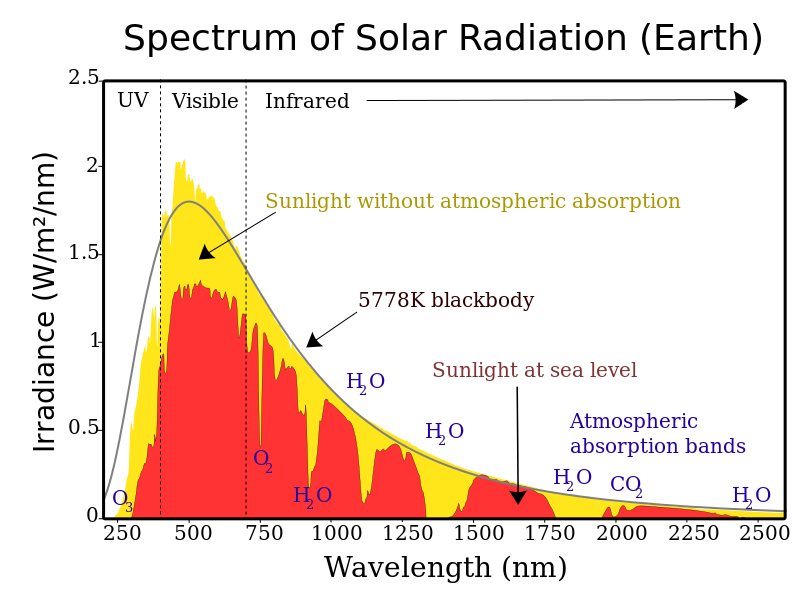
\includegraphics[height=8cm]{pbr/solar_spectrum.png}
  \caption{Widmo światła widzialnego emitowanego przez Słońce. Źródło: \url{https://en.wikipedia.org/wiki/Sunlight}}
  \label{fig:solar_spectrum}
\end{figure}

Oddziaływanie światła z materią opisuje wielkość nazywana współczynnikiem załamania $n$. Współczynnik załamania mówi nam, jak materia wpływa na prędkość światła oraz w postaci rozszerzonej w której współczynnik jest wartością zespoloną pozwala obliczyć jak dużo światła dany ośrodek absorbuje. Podstawowym wzorem na $n$ jest:
\[
    n = \frac{c}{v}
\]
gdzie $c$ jest prędkością światła w próżni ($\SI{2.998e8}{\meter\per\second}$), a $v$ prędkością fazową fali, czyli prędkością z jaką faza propaguje się w przestrzeni.

Najprostszym rodzajem ośrodka jest medium jednorodne, które ma jednolitą strukturę wewnętrzną o stałym współczynniku załamania. Na skutek tego prędkość światła w każdym punkcie i dowolnym kierunku jest jednakowa. W takim przypadku światło w ośrodku porusza się w linii prostej. Najlepszym przykładem ośrodka tego typu jest próżnia. Mimo braku zmiany kierunku w większości ośrodków następuje utrata energii na skutek absorpcji, wynikającej ze zderzeń z atomami materii. Nawet niewielki stopień utraty energii może skutkować całkowitym jej pochłonięciem na większym dystansie np. pod wodą. Innym przykładem medium jednorodnego o niskiej absorpcji jest szkło i powietrze.

Ośrodek niejednorodny jest ośrodkiem o niejednorodnej strukturze wewnętrznej, w której prędkość światła jest zależna od kierunku lub badanego miejsca - w związku z czym współczynnik załamania jest zależny od pozycji w ośrodku. Jeżeli w otoczeniu danego punktu współczynnik załamania zmienia się to promień przechodzący przez ten punkt zmieni swój kierunek. W przypadku ciągłej zmiany współczynnika promień zostanie zagięty, jednak dla nieciągłości wiązka zostanie podzielona na dwie części - na część refrakcyjną oraz odbitą. Część odbita nie opuści obecnego ośrodka, lecz zmieni kierunek i wróci do jego wnętrza. Część refrakcyjna natomiast zagnie się oraz przejdzie do drugiego ośrodka. 

W bardzo różnorodnych strukturach może dojść do sytuacji, w której na skutek dużej ilości nieciągłości lub znacznych wahań współczynnika załamania światło wymiesza się tak, że promienie będą podążały w losowych kierunkach. Takie zjawisko nazywamy rozpraszaniem (ang. \textit{scattering}). Przykładem substancji w której łatwo je zaobserwować jest mleko.

Warto w tym miejscu zastanowić się nad znaczeniem skali dla rozpraszania światła. Małe zaburzenia w niewielkim otoczeniu mogą nie mieć dużego wpływu na fale świetlne, lecz w dużej skali nie mogą zostać pominięte. Czyste powietrze nie powoduje mieszania się światła na krótkich dystansach, jednak nawet taki ośrodek powoduje znaczne rozproszenie, gdy bierzemy pod uwagę sceny w których można dostrzec punkty leżące wiele kilometrów od obserwatora. 

Oprócz jednorodności lub niejednorodności możemy podzielić substancje na trzy główne kategorie, są to:

\begin{itemize}
	\item przewodniki (metale) - materiały dobrze przewodzące prąd elektryczny, przykładami przewodników są: grafit, żelazo, stal, aluminium, złoto, miedź,
    
	\item izolatory (dielektryki) - materiały w których prąd elektryczny przewodzony jest bardzo słabo, jest to rezultatem niskiej koncentracji ładunków swobodnych i/lub zbyt małej ich ruchliwości; przykładami dielektryków są szkło, ceramika, tworzywa sztuczne, suche drewno, powietrze,
	
	\item półprzewodniki - substancje, dla których przewodnictwo prądowe może być zmieniane w szerokim zakresie. Ze względu na ich rzadkie występowanie w codziennym otoczeniu (poza środowiskami laboratoryjnymi), nie będziemy ich brać pod uwagę. W przypadku konieczności wymodelowania materiału półprzewodnikowego możemy zbudować wystarczający w wielu przypadkach model będący interpolacją między przewodnikiem a izolatorem.
\end{itemize}

Metale oraz dielektryki posiadają kilka szczególnych właściwości, które muszą zostać wzięte pod uwagę podczas obliczeń. Różnice zostaną przedstawione nieco później w tym rozdziale.

Zrozumienie zachowania wiązki światła po zderzeniu z idealnie równą powierzchnią jest fundamentem całej dziedziny metod opartych na prawach fizycznych. Dopóki nie wprowadzimy pojęcia chropowatości będziemy zakładać, że analizowana powierzchnia jest optycznie gładka, to znaczy, że wszystkie nierówności na tej powierzchni są mniejsze niż długość aktualnie analizowanej fali (mniejsze niż $400-700$nm), przez co możemy przyjąć, że nie wpływają one w żaden sposób na zachowanie promieni.

Dla uproszczenia objaśnień będziemy również zakładać, że analizowany materiał nie emituje światła. Dodanie emisji energii nie powinno stanowić żadnego problemu po zbudowaniu modelu dla interakcji z zewnętrznymi źródłami światła.

Wiązka światła podczas zderzenia z powierzchnią (dokładniej, przy przejściu z jednego ośrodka do drugiego, w miejscu w którym występuje nieciągłość współczynnika załamania) rozdziela się na dwie części: część odbitą od powierzchni oraz załamaną (część, która ulega refrakcji).

Reflektancją powierzchniową $\mathbb{R}^{\text{surf}}$ \cite{pbr_games_siggraph} nazywamy stosunek natężenia światła odbitego $I_o$ do światła przychodzącego $I_i$ w danym punkcie dla danej długości fali $\lambda$:
\[
	\mathbb{R}^{\text{surf}}(\lambda) = \frac{
        I_o
    }{
        I_i
    } \in \left[
        0, 1 
    \right]
\]

Reflektancja powierzchniowa zależna jest również od kąta padania promienia oraz długości fali. Reflektancję dla kąta padania równego $\ang{0}$ będziemy oznaczać poprzez $\mathbb{R}^{\text{surf}}_{0}$ - ta wartość bardzo często używana jest jako wartość bazowa dla modeli przybliżających współczynnik reflektancji dla wszystkich kątów. 

Różnice między metalami, a izolatorami zaczynają być widoczne przy analizie reflektancji powierzchniowej. Wartość $\mathbb{R}^{\text{surf}}_{0}$ dla izolatorów zwykle nie przekracza 6\%. Sytuacja wygląda zupełnie inaczej w świecie metali, współczynnik reflektancji powierzchniowej dla kierunku zgodnego z normalną tej powierzchni ($\mathbb{R}^{\text{surf}}_{0}$) jest zazwyczaj wyższy niż 50\%.

Część energii, która uległa refrakcji, wchodzi wgłąb, gdzie zachodzą kolejne kolizje z atomami materii, przez co znów dochodzi do wyżej wspomnianego zjawiska podziału promienia, tym razem we wnętrzu badanego ciała. Część tego światła może wydostać się ponownie z obiektu do ośrodka źródłowego, pozostała część zostanie pochłonięta i zamieniona na inne rodzaje energii np. ciepło.

Ilość światła, które wydostaje się z powrotem z wnętrza ciała jest zależna od rodzaju substancji z której jest wykonany obiekt. Dla metali część energii, która dostaje się do wnętrza zostaje bardzo szybko pochłonięta przez wolne elektrony i zamieniona na ciepło. Z tego względu światło, które ulega refrakcji nie wydostanie się z tego metalu. Wnioskiem jest to, że na wygląd metali wpływają jedynie promienie, które zostają odbite od jego powierzchni. Dla dielektryków sytuacja wygląda inaczej, ze względu na budowę atomową światło nie jest pochłaniane w dużym stopniu i bardzo często jest uwolnione w innym miejscu ciała.

W modelach matematycznych, wymienionych w tej pracy, zakładamy, że ponowne wyjście energii, która była poddana refrakcji następuje lokalnie tzn. we fragmencie powierzchni, która przypada na obecnie generowany piksel, w którym promień zderzył się z obiektem (rys. \ref{fig:ReflectionRefraction}).

% Rysunek odbicia z płaską powierzchnią (model uproszczony)
\begin{figure}[h]
  \centering
  \begin{tikzpicture}
    %\draw[help lines] (-5,-1) grid (5,5);
    \draw [thick] (-5.0,0.0) -- (5.0,0.0);

    % Specular
    \foreach \i in {0,...,5} {
      \pgfmathtruncatemacro{\angle}{90+30+(\i / 5) * 30};
      \draw [-Triangle, blue] (0,0) -- ( {3*cos(\angle)}, {3*sin(\angle)} );
    }

    % Diffuse
    \foreach \i in {1,...,15} {
      \pgfmathtruncatemacro{\angle}{(\i / 16) * 180};
      \draw [-Triangle, gray] (0,0) -- ( {2*cos(\angle)}, {2*sin(\angle)} );
    }

    \draw [fill] (2,2) circle [radius=0.05] node [above] {\Large\faLightbulbO};
    \draw [-{Triangle[scale=2]}] (2,2) -- (0,0);
  \end{tikzpicture}
  \caption{Przybliżony model interakcji wiązki światła z powierzchnią. Niebieskie strzałki reprezentują promienie odbite od powierzchni, szare zaś promienie, które dostały się do wnętrza obiektu i na skutek zderzeń wewnętrznych wydostały się z powrotem na zewnątrz. Opracowanie własne.}
  \label{fig:ReflectionRefraction}
\end{figure}

Istnieją techniki które biorą pod uwagę możliwość ucieczki energii w dalej położonym miejscu, ale skomplikowałyby one rozważania na których skupia się ta praca. Takie techniki muszą operować globalnie i zakładać możliwość wpływu fragmentów powierzchni obiektu na inne obszary. Wymagane są one, do uzyskania realistycznych obrazów, w których pojawiają się materiały takie jak skóra, wosk, dla których rozproszenie podpowierzchniowe jest wyraźnie widoczne. Zauważmy znowu, że rozważanie tego, czy dany materiał wymaga globalnej metody na wyznaczenie ucieczki światła z wnętrza materii jest zależne od skali. Jeżeli będziemy obserwować plastik, który w wymiarze standardowym dla gier nie wykazuje żadnych widocznych ,,interakcji'' między pikselami, nie oznacza to, że będzie tak również dla bardzo dużego przybliżenia tej powierzchni. Podobnie rozpalona woskowa świeczka lub marmurowa rzeźba zmniejszona do bardzo małych rozmiarów, nie będzie wykazywała istnienia takiego zjawiska.

Reflektancja powierzchniowa nie bierze pod uwagę światła uciekającego z wnętrza ciała. Dlatego też, zdefiniujemy dodatkowe pojęcie, które będziemy nazywać reflektancją ciała lub objętości (ang. \textit{body/volume reflectance}). Definicja będzie analogiczna do poprzedniej: reflektancją objętośći $\mathbb{R}^{\textit{vol}}$ nazywamy stosunek ilości światła wychodzącego do przychodzącego w bardzo małym obszarze wokół danego punktu. W przeciwieństwie do reflektancji powierzchniowej, wartość reflektancji objętościowej jest bardzo zróżnicowana, współczynnik ten dla śniegu wynosi około 80\%, dla kamienia około 20\%, a dla węgla blisko 0\%.

Zauważmy, że w przypadku braku emisji oraz przy lokalnej ucieczce światła z materii energia, która dociera do obserwatora musi być mniejsza lub równa energii przychodzącej wiązki światła - ta właściwość jest jednym z filarów modeli opartych na zjawiskach fizycznych.

\begin{figure}[ht]
  \centering
  \begin{tikzpicture}
    %\draw[help lines] (-5,-1) grid (5,5);

		\coordinate (left) at (-3,0);
		\coordinate (right) at (3,0);
    \draw [ultra thick] (left) -- (right);

		\coordinate (normal) at (0,3);
		\coordinate (invnormal) at (0,-3);

    \draw  [-{Triangle[scale=2]}] (invnormal) -- (normal) node [above] {$N$};

		\coordinate (orig) at (0,0);
		\coordinate (light) at (45:3);
		\coordinate (reflection) at (135:3);
		\coordinate (refraction) at (205:3);

    \draw  [-{Triangle[scale=2]}] (orig) -- (reflection)
      node [midway, above] {$r$};
    \draw  [-{Triangle[scale=2]}] (orig) -- (refraction)
      node [midway, above] {$t$};
    \draw  [-{Triangle[scale=2]}] (light) -- (orig);

    \draw pic[draw=black, <->, "$\alpha_i$", angle eccentricity=1.5]
			{angle = light--orig--normal};

    \draw pic[draw=black, <->, "$\alpha_r$", angle eccentricity=1.5]
			{angle = normal--orig--reflection};

    \draw pic[draw=black, <->, "$\beta$", angle eccentricity=1.5]
			{angle = refraction--orig--invnormal};

    \node at (2.8,+0.25) {$n_1$};
    \node at (2.8,-0.25) {$n_2$};

    \draw [fill] (light) circle [radius=0.05] node [above] {\Large\faLightbulbO};

  \end{tikzpicture}
  \caption{Przybliżony model interakcji wiązki światła z optycznie gładką powierzchnią. Opracowanie własne.}
  \label{fig:ReflectionRefractionDetailed}
\end{figure}

Do określenia tego, ile i w jaki sposób wiązka światła będzie oddziaływać z powierzchnią poprzez odbicie lub refrakcję, będziemy potrzebować kilku podstawowych praw fizycznych. Notacja wykorzystana we wzorach jest zgodna ze schematem z rys. \ref{fig:ReflectionRefractionDetailed}.

Podstawowym prawem wykorzystywanym do analizy zachowania wiązki światła jest prawo wiążące kąt padania oraz kąt odbicia promienia. Kąty padania wiązki światła $\alpha_i$ i jej odbicia $\alpha_r$ od płaszczyzny (zatem od idealnie gładkiej powierzchni) są równe ($\alpha_i = \alpha_r = \alpha$).


Zmiana kierunku promienia światła przy przejściu przez granicę dwóch ośrodków jednorodnych o współczynnikach załamania $n_1, n_2$ opisana jest równaniem Snella:
\[
\frac{\sin\alpha}{\sin\beta} =
  \frac{n_2}{n_1} = n_{21}
\]

Stosunek energii wiązki światła odbitego do załamanego opisany jest równaniami Fresnela, będących rozwiązaniem równań Maxwella dla fal świetlnych przechodzących przez jednorodne ośrodki o różnych współczynnikach załamania przez idealnie płaską granicę. W tej pracy nie będziemy korzystać bezpośrednio z równań Fresnela, lecz z ich aproksymacji, w szczególności z aproksymacji Schlicka. Współczynnik Fresnela, jego znaczenie i opis aproksymacji zostanie przedstawione dalej w tym rozdziale.

Prawo odbicia światła, równanie Snella oraz równania Fresnela pozwalają nam na opis zachowania światła wystarczający do zastosowań w grafice czasu rzeczywistego.

W naturze mało który materiał jest optycznie idealnym lustrem (tak abyśmy mogli zastosować tutaj uproszczone równania Fresnela), w odpowiednio dużym przybliżeniu realnych pozornie gładkich powierzchni zauważymy nierówności niedostrzegalne gołym okiem, a jednocześnie wpływające znaczące na ogólny wygląd powierzchni (rys. \ref{fig:Microstructure}). Im większa jest nierówność, tym większe jest zróżnicowanie normalnych w tym otoczeniu. W związku z tym światło się bardziej miesza i refleksy są coraz mniej wyraźne. Nierówności powierzchni wpływające na jej wygląd, lecz nieobserwowalne w badanej skali, będziemy nazywać mikrogeometrią lub mikrostrukturą.

\begin{figure}[ht]
  \centering
  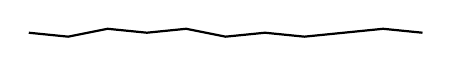
\begin{tikzpicture}
    \draw [thick]
      (0.0,0.15) --
      (0.5,0.10) --
      (1.0,0.20) --
      (1.5,0.15) --
      (2.0,0.20) --
      (2.5,0.10) --
      (3.0,0.15) --
      (3.5,0.10) --
      (4.0,0.15) --
      (4.5,0.20) --
      (5.0,0.15);
  \end{tikzpicture}
  \hspace{0.5cm}
  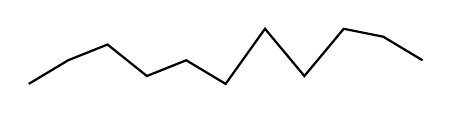
\begin{tikzpicture}
    \draw [thick]
      (0.0,0.1) --
      (0.5,0.4) --
      (1.0,0.6) --
      (1.5,0.2) --
      (2.0,0.4) --
      (2.5,0.1) --
      (3.0,0.8) --
      (3.5,0.2) --
      (4.0,0.8) --
      (4.5,0.7) --
      (5.0,0.4);
  \end{tikzpicture}
  \vspace{0.25cm}
  \caption{Mikrostruktury powierzchni o różnej chropowatości. Opracowanie własne.}
	\label{fig:Microstructure}
\end{figure}

Warto zauważyć, że nawet jeżeli wiązka światła odbija się w kierunku obserwatora nie oznacza to, że wyjdzie z otoczenia powierzchni i do niego trafi. Mała nierówność może spowodować zasłonięcie obserwatora z perspektywy punktu zderzenia i odbić się ponownie w zupełnie innym kierunku. Będziemy wtedy mówić o maskowaniu (ang. \textit{masking}). Modele bazujące na mikro-powierzchniach zazwyczaj nie biorą pod uwagę odbić wielokrotnych i to takimi modelami odbić jednokrotnych (ang. \textit{single-bounce models}) będziemy się zajmować. Wielokrotne odbicie w mikrostrukturze (ang. \textit{multiple-bounce model}) jest wciąż problemem otwartym, nie istnieją zrozumiałe i powszechnie akceptowane modele opisujące to zjawisko.

Możliwa jest również sytuacja odwrotna, w której dany punkt może być teoretycznie zaobserwowany przez obserwatora, ale światło nie dociera do tego punktu na skutek przysłaniania źródła światła przez sam obiekt (samo-zacienianie, ang. \textit{shadowing}).

\missingfigure{Rysunek samozaciemniania moze tutaj?}

\section{Podstawowe pojęcia radiometryczne}

Rozpocznijmy od podstawowego budulca wiązki światła - fotonu. Energię pojedynczego fotonu o długości fali $\lambda$ możemy obliczyć przy użyciu wzoru:
\[ 
    Q = \frac{hc}{\lambda} 
\]
\noindent gdzie $h$ jest stałą Plancka ($\SI{6.62620e-34}{\joule\per\second}$), a $c$ prędkością światła w próżni. Wszystkie kolejne miary przedstawione w tej sekcji są funkcją długości fali.

Strumień promieniowania (inaczej moc promieniowania, ang. \textit{radiant flux}) to całkowita ilość energii przechodzącej przez określoną powierzchnię w czasie jednostkowym. Powyższe pojęcie dotyczy wszystkich fal elektromagmetycznych, zatem jest ono poprawne również dla światła. Jednostką strumienia promieniowania jest Watt ($\si{\watt}$).
\[
\Phi = 
    \lim_{\Delta t \rightarrow 0}{
        \frac{\Delta Q}{\Delta t}
    } 
    = \frac{\dd Q}{\dd t}
\]


Radiancją wyjściową (ang. \textit{radiant exitance, radiosity}) $B$ nazywamy wyemitowany strumień promieniowania $\Phi_{e}$ przez powierzchnię na jej powierzchnię jednostkową:
\[
B(p) = 
    \lim_{\Delta \rightarrow 0}{
        \frac{\Delta \Phi_{e}(p)}{\Delta A}
    } 
    = \frac{\dd \Phi_{e}}{\dd A}
\]  

Irradiancją (ang. \textit{irradiance}) nazywamy strumień promieniowania przychodzącego $\Phi$ na jednostkę powierzchni:
\[
E(p) =
    \lim_{\Delta \rightarrow 0} {
        \frac{\Delta \Phi(p)}{\Delta A}
    } =
    \frac{\dd \Phi(p)}{\dd A}
\]

Oczywiście całkując irradiancję na powierzchni otrzymamy z powrotem strumień promieniowania:
\[
\Phi = \int_{A} {
    E(p)
    \dd A
}
\]

W tym miejscu warto zauważyć, że jeżeli powierzchnia $A$ jest nachylona do
strumienia światła $\Phi$ pod pewnym kątem $\alpha$, to irradiancja zmienia się
proporcjonalnie do czynnika $\cos \alpha$. Wynika to z faktu, że obszar na
który padają promienie emitowane przez źródło światła w kierunku prostopadłym
do powierzchni tego źródła, jest zależny od kąta pod którym nachylona jest
powierzchnia (uzasadnienie graficzne znajduje się na rys. \ref{fig:SourceLightAngle}). Powierzchnia ta jest odwrotnie proporcjonalna do czynnika $\cos \alpha$, zatem dzieląc przez powierzchnię otrzymujemy zależność wprost proporcjonalną dla irradiancji.

\begin{figure}[ht]
  \centering
  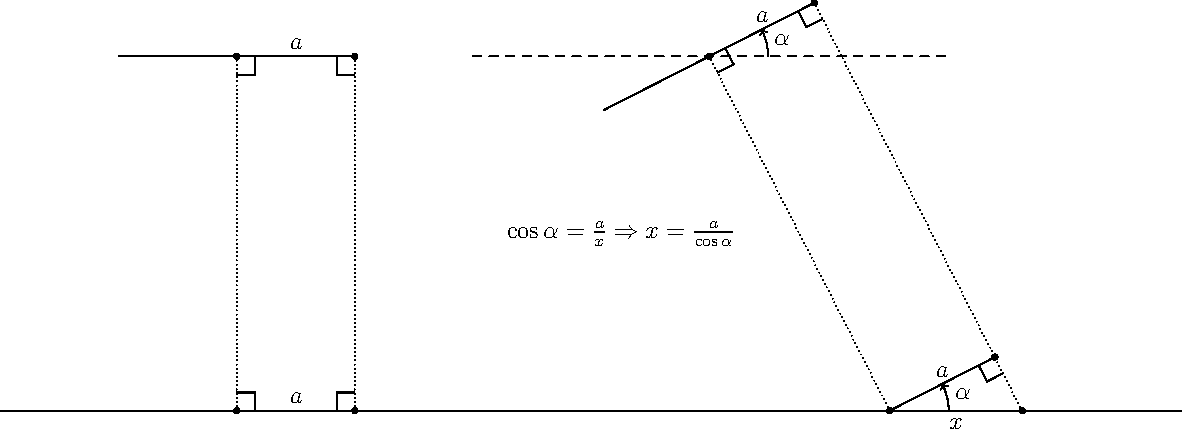
\includegraphics[height=5.5cm]{pbr/light_angle.pdf}
  \caption{Wpływ kąta na powierzchnię na którą oddziaływuje światło. Opracowanie własne.}
  \label{fig:SourceLightAngle}
\end{figure}

W przypadku jednorodnym irradiancję możemy zdefiniować jako średnią moc
promieniowania na pewnej skończonej powierzchni $A$:
\[
    E = \frac{\Phi}{A}
\]

\begin{example}
  Irradiancja dla światła punktowego w punkcie $p$ na sferze o
  promieniu $r$ o środku w tym właśnie punkcie $p$ wynosi:
  \[
    E = \frac{\Phi}{4 \pi r^2}
  \]
\end{example}

Kątem planarnym obiektu geometrycznego $G$ z punktu $p$ (rys. \ref{fig:PlanarAngle}) nazywamy kąt wyznaczony przez dwie półproste rozpoczynające się w punkcie $p$, określające minimalny obszar zawierający obiekt $G$. Miarą kąta planarnego jest \textit{radian} (\si{\radian}). Inaczej mówiąc, kąt jest ciągłym zbiorem kierunków na płaszczyznie, a jego rozmiar jest równy długości łuku wyznaczonego przez wektory jednostkowe odpowiadające tym kierunkom.

% Rysunek kąta geometrycznego
\begin{figure}[ht]
  \centering
  \begin{tikzpicture}
    \coordinate (orig) at (0,0);
    \coordinate (left) at (1,3);
    \coordinate (right) at (5,2);
    \draw (2,1) -- (left) -- (2,4) -- (right) -- (2,1);
    \draw [dashed] (left)--(orig)--(right);
    \draw [fill] (orig) circle [radius=0.08] node [below] {$p$};
    \draw pic[draw=black, <->, "$\theta$", angle eccentricity=1.5] {angle = right--orig--left};
  \end{tikzpicture}
  \caption{Kąt planarny obiektu geometrycznego. Opracowanie własne.}
  \label{fig:PlanarAngle}
\end{figure}

Kąt bryłowy jest rozszerzeniem kąta planarnego do trzech wymiarów. Kątem bryłowym $A$ nazywamy ciągły zbiór kierunków w przestrzeni trójwymiarowej, mierzony polem powierzchni obszaru zdefiniowanego przez wektory jednostkowe odpowiadające tym kierunkom. Kątem bryłowym możemy też nazwać powierzchnię rzutu trójwymiarowego obiektu geometrycznego $G$ na sferę jednostkową o środku w punkcie $p$. Jest on mierzony w steradianach (\si{\steradian}). Kąt bryłowy całej sfery jednostkowej wynosi $\SI{4\pi}{\steradian}$.

% Rysunek kąta bryłowego
\begin{figure}[ht]
  \centering
  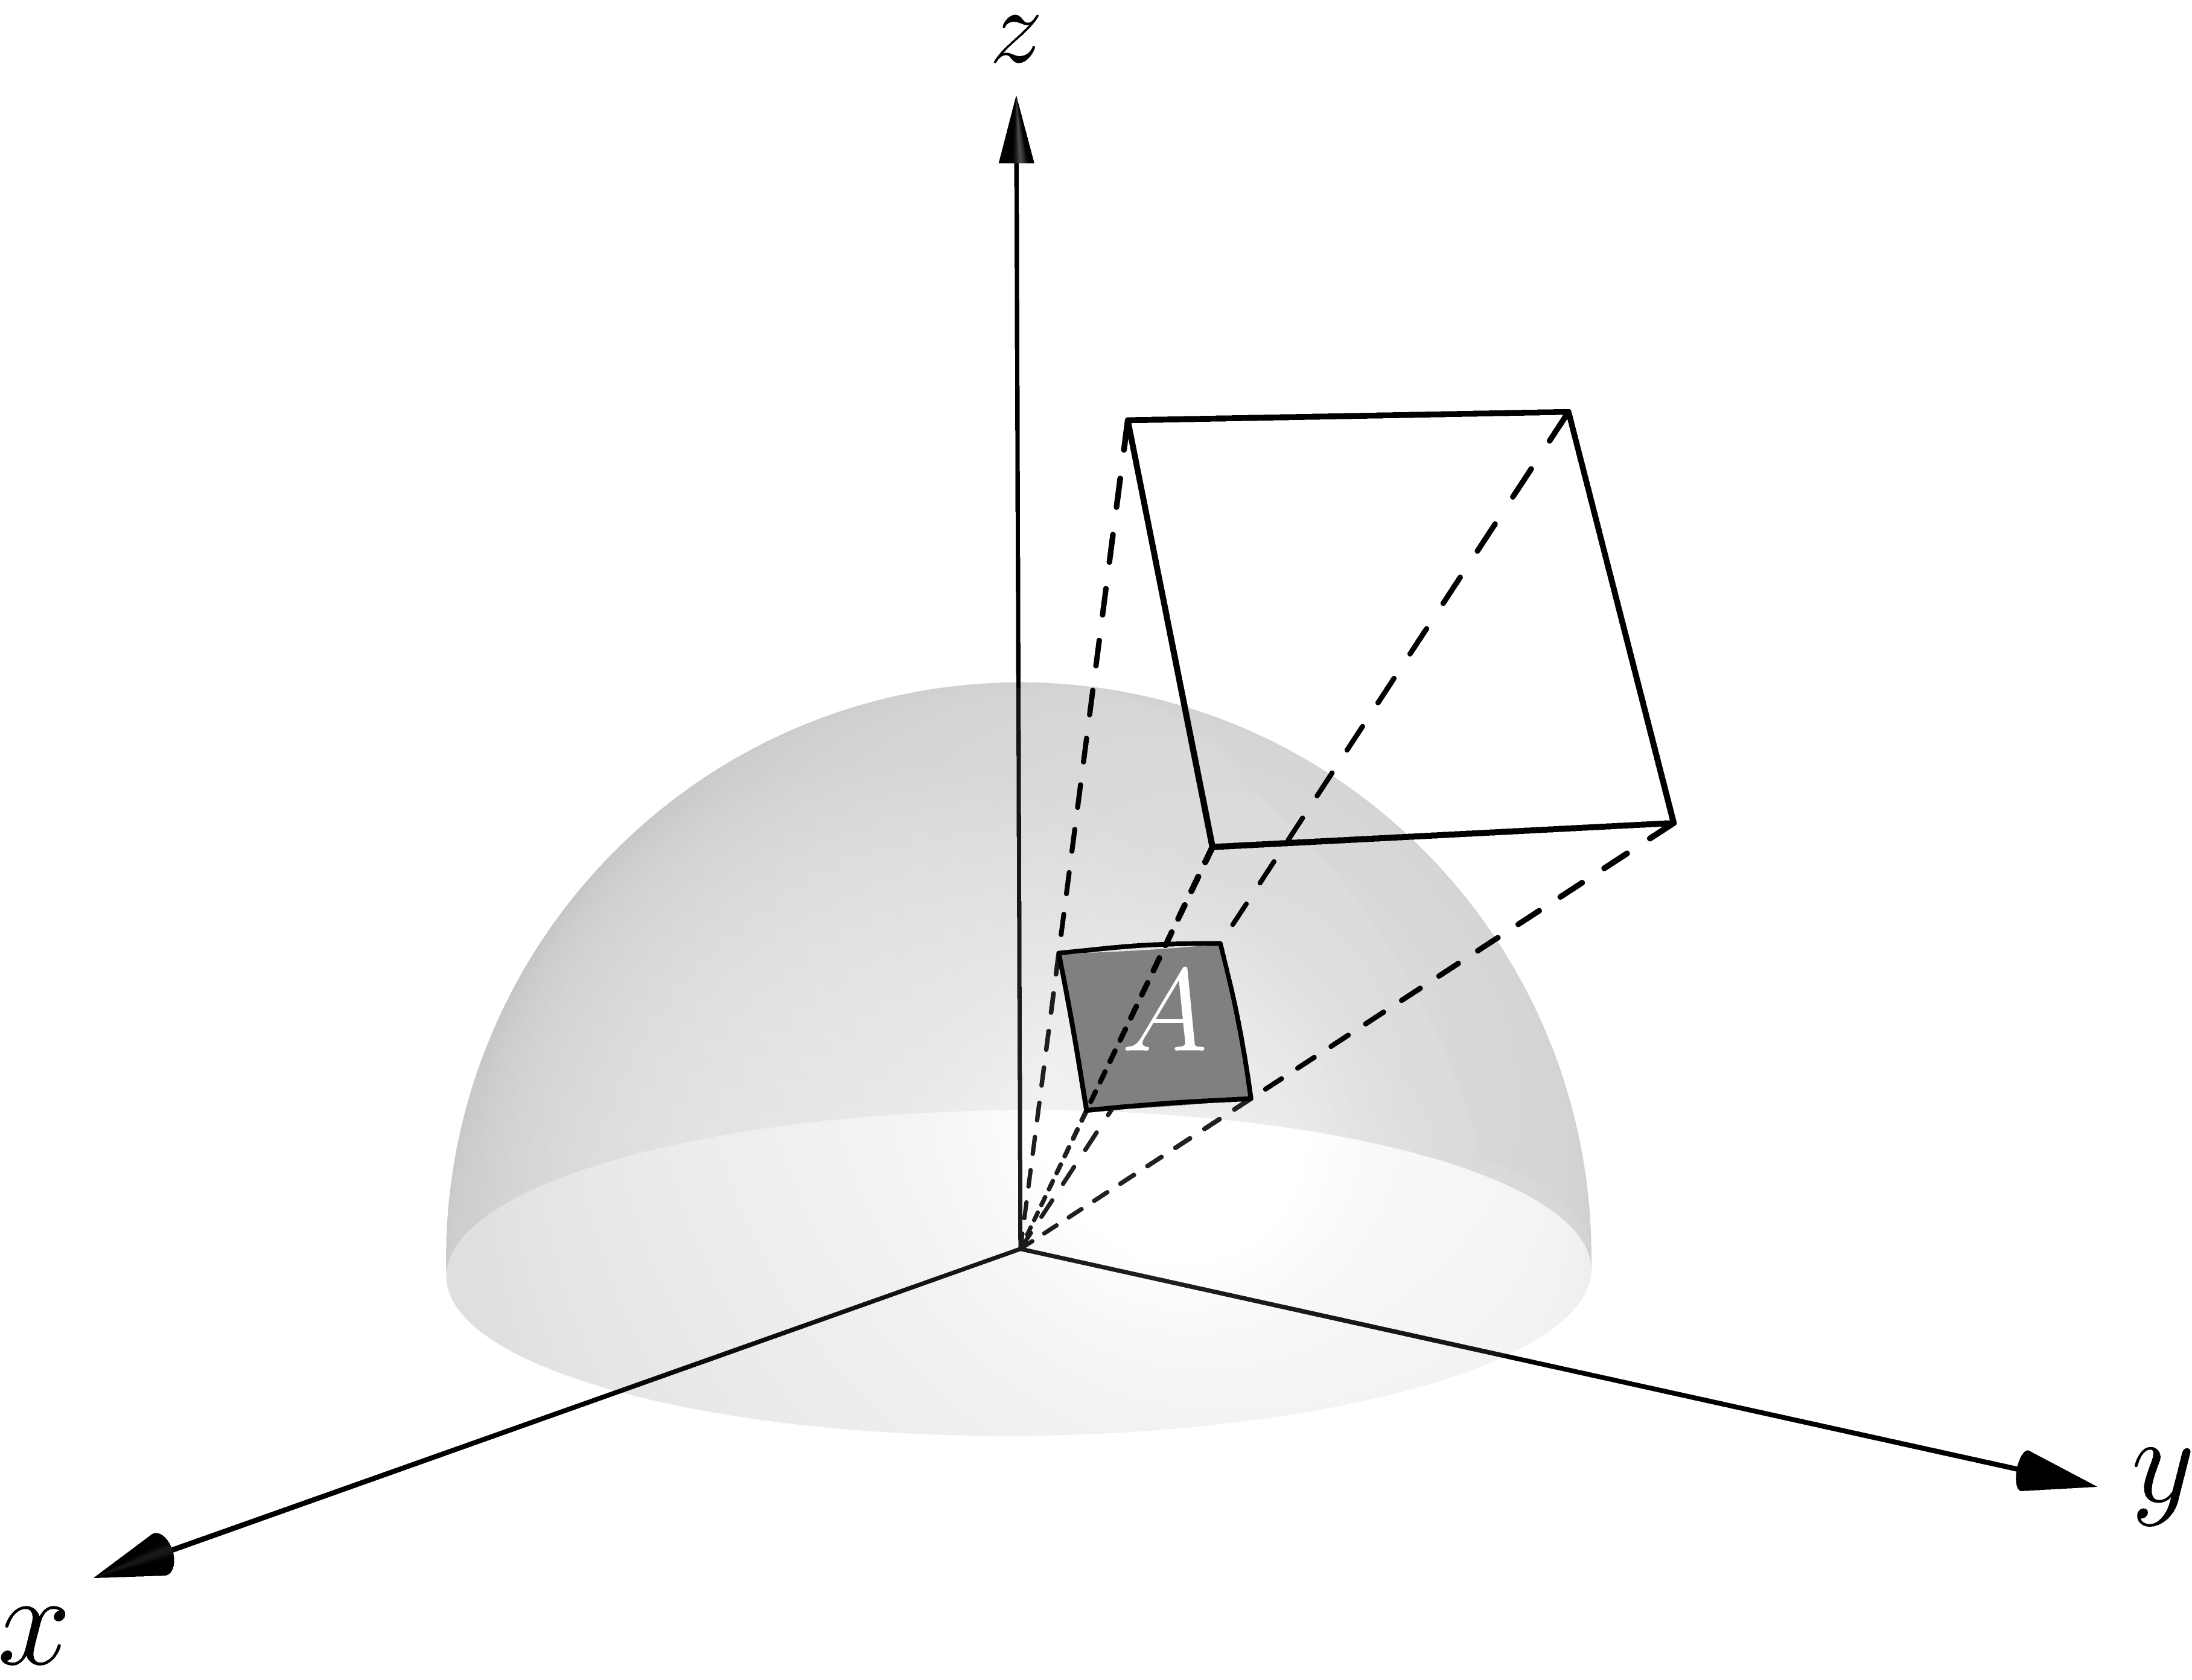
\includegraphics[height=5cm]{pbr/solid_angle.png}
  \caption{Kąt bryłowy powierzchni. Opracowanie własne.}
  \label{fig:SolidAngle}
\end{figure}

Kolejną miarą energii jest intensywność źródła (ang. \textit{intensity}), która reprezentuje rozkład gęstości mocy światła na kierunkach \cite[str. 328]{pbrt}. Warto na wstępie zauważyć, że intensywność ma sens, tylko i wyłącznie dla teoretycznych świateł punktowych lub bardzo odległych, które możemy traktować jako kierunkowe, ze względu na sposób pomiaru kąta. Wartość tą możemy zdefiniować w następujący sposób:
\begin{gather*}
  I = \lim_{\Delta\omega \rightarrow 0} {
    \frac{\Delta\Phi}{\Delta\omega}
  } = \frac{\dd \Phi}{\dd \omega} \\
  \Phi = \int_{\Omega} {I(\omega) \dd \omega}
\end{gather*}
\noindent gdzie przez $\omega$ rozumiemy wektor określający kierunek ze środka
jednostkowej sfery do punktu leżącego na jej brzegu.

Dla przykładu intensywność teoretycznego jednorodnego światła punktowego wynosi:
\[
  I = \frac{\Phi}{4\pi}
\]

Poprzez $E_{\omega}$ oznaczmy irradiancję hipotetycznej powierzchni
prostopadłej do kierunku $\omega$. Luminancją energetyczną (inaczej radiancją, ang. \textit{radiance}) $L$ nazywamy miarę irradiancji $E_{\omega}$ w odniesieniu do kąta bryłowego:
\[
L(p, \omega) = \lim_{\Delta\omega \rightarrow 0} {
  \frac{\Delta E_{\omega} (p)}{\Delta\omega}
} =
\frac{\dd E_{\omega}(p)}{\dd \omega}
\]

Bardzo ważną obserwacją jest to, że luminancja energetyczna nie jest mierzona względem irradiancji powierzchni na której leży punkt $p$, ma to na celu wyeliminowanie czynnika $\cos \alpha$ z definicji \cite[str. 339]{pbrt}. Jednostką radiancji jest gęstość energii na jednostkę powierzchni na jednostkę kąta bryłowego. Luminancję energetyczną możemy interpretować jako miarę ilości światła wzdłuż jednego promienia.

Irradiancję (tutaj względem normalnej makro-powierzchni) możemy odzyskać całkując luminancję energetyczną względem makro-powierzchni (stąd czynnik $\cos\theta$):
\begin{gather*}
    \dd E = L(p, \omega) \cos\theta \dd \omega \\
    E = \int_{\Omega_H}{L(p, \omega) \cos\theta \dd \omega}
\end{gather*}

Dwukierunkową funkcją rozkładu odbicia (ang. \textit{Bidirectional Reflectance Distribution Function, BRDF}) nazywamy stosunek irradiancji do odbitej radiancji:
\[
f_r(\omega_i, \omega_o) = \frac{
    \dd L_{o}(\omega_o)
}{
    \dd E(\omega_i)
}
\]
\noindent Jednostką BRDF jest $\si[per-mode=reciprocal]{\per\steradian}$.

\section{Równanie renderingu}

\textbf{Równanie renderingu} to równanie całkowe, określające radiancję wychodzącą z danego punktu $p$ w danym kierunku $\omega_o$ znając radiancję przychodzącą do tego punktu. Równanie te możemy
wyprowadzić z poprzednio przedstawionych definicji:
\begin{gather*}
    f_r(\omega_i, \omega_o) = \frac{
        \dd L_{o}(\omega_o)
    }{
        \dd E(\omega_i)
    } \Rightarrow 
    \dd L_{o}(\omega_o) =  f_r(\omega_i, \omega_o) \dd E(\omega_i) \\
    \dd E(\omega_i) = L_i(p, \omega) \cos\theta \dd\omega
\end{gather*}

Podstawiając drugie równanie do pierwszego i całkując otrzymujemy:
\[
  L_{o}(\omega_o) =
  \int_{\Omega} {
    f_r(p, \omega_i, \omega_o)
    L_i(\omega_i)
    (n \cdot \omega_i)
    \dd{\omega_i}
  }
\]

\noindent gdzie poszczególne składowe to:

\begin{itemize}

  \item $L_i(\omega_i)$ - radiancja przychodząca z kierunku $\omega_i$,

  \item $\Omega$ - jednostkowa półsfera wyznaczająca dziedzinę wszystkich
    możliwych kierunków przychodzących $\omega_i$,

  \item $f_{r}(p, \omega_i, \omega_o)$ - dwukierunkowa funkcja rozkładu odbicia wyznaczająca jaka część energii przybywającej z kierunku $\omega_i$ zostanie wysłana w zadanym kierunku $\omega_o$.

\end{itemize}

Bardzo często wykorzystywaną formą tego równania jest postać z parametryzacją polarną kątami $\phi$ i $\theta$. W takim przypadku $\dd \omega$ jest równe $\sin\theta \dd\theta \dd\phi$ \cite{wolfram_solidangle} stąd uzyskujemy:
\[
L_{o}(\theta_o, \phi_o) = \int_{0}^{2\pi} \int_{0}^{\frac{\pi}{2}} {
	f(\theta_i, \phi_i, \theta_o, \phi_o)L(\theta_i, \phi_i) \cos\theta_i \sin\theta_i
} \dd\theta_i \dd\phi_i
\]

\noindent Postać ta jest szczególnie istotna w zastosowaniach praktycznych.

\section{Dwukierunkowa funkcja rozkładu odbicia}

Dwukierunkowa funkcja rozkładu odbicia (ang. \textit{Bidirectional Reflectance Distribution Function, BRDF}) musi spełniać dwa warunki by była fizycznie wiarygodna. Po pierwsze, funkcja BRDF musi być niezależna od kolejności parametrów, odwrócenie wszystkich kierunków promieni powinno dać nam dokładnie ten sam wynik\footnote{Zależność tą można w literaturze anglojęzycznej spotkać pod nazwą \textit{Helmholtz reciprocity}.}:
\[
  \forall{\omega_i, \omega_o \in \Omega} \quad
  f_r(\omega_i, \omega_o) = f_r(\omega_o, \omega_i)
\]

Po drugie, funkcja BRDF nie może przekazywać do otoczenia więcej światła niż otrzymuje (pamiętajmy o założeniu braku emisji). Kierunkowa reflektancja półsferyczna (ang. \textit{directional-hemispherical reflectance}) $R(\omega_i)$ jest kolejną funkcją związaną z BRDF mierzącą ile energii przychodzącej z danego kierunku $\omega_i$ zostanie odbite w jakimkolwiek innym kierunku. Inaczej mówiąc, mierzy ona straty lub zyski energii dla danego kierunku wejściowego. Zauważmy, że dla modeli spełniających warunek zachowania energii wartość ta musi być w przedziale $\left[0,1\right]$ dla każdej długości fali $\lambda$ i kierunku przychodzącego $\omega_o$. Funkcja ta zdefiniowana jest w sposób następujący \cite{RealTimeRendering2008}:
\[
  R(\omega_i) 
  = \frac{\dd B}{\dd E(\omega_i)} 
  = \int_{\Omega} {
    f_r(\omega_i, \omega_o)
    (n \cdot \omega_o)
    \dd \omega_o
  }
\]

W tym miejscu warto wprowadzić kolejną wielkość nazywaną albedo lub bi-półsferycznym współczynnikiem odbicia (ang. \textit{bihemispherical reflectance, albedo}) zdefiniowaną jako stosunek całkowitej radiancji wyjściowej do irradiancji.
\[
    \rho = \frac{B}{E} = \frac{1}{\pi} \int_{\Omega}{
        R(\omega_i) \cos\theta_i d\omega_i
    }
    = \frac{1}{\pi} \int_{\Omega} \int_{\Omega} {
        f_r(\omega_i, \omega_o) 
        \cos\theta_i 
        \cos\theta_o 
        \dd\omega_i 
        \dd\omega_o
    }
    \in \left[0, 1\right]
\]

Albedo jest bardzo użyteczną miarą, którą można interpretować jako ogólny stopień refleksywności danej powierzchni. Parametr ten bardzo często jest wykorzystywany jako parametr wejściowy systemu oświetlenia.

Cała funkcja BRDF zwykle zawiera część opisującą reflektancję powierzchniową (odbitą, ang. \textit{specular}) oraz część dla reflektancji ciała (rozproszoną, ang. \textit{diffuse}), przez co większość modeli rozdziela je i analizuje osobno lub definiuje tylko jeden fragment możliwy do wykorzystania z innym. Do podziału wiązki światła przy zderzeniu najczęściej używane są równania Fresnela.

Istnieje bardzo dużo róznych modeli BRDF \cite{brdf_overview}, my zajmiemy się natomiast kilkoma wybranymi.

\subsection{Model Lamberta}

Najprostszą funkcją BRDF jest rozkład jednorodny, niezależny od kąta obserwacji. Taka funkcja, nazywana rozkładem lambertowskim, jest opisana poniższym równaniem:
\[
  f_r = \frac{\rho}{\pi}
\]
\noindent gdzie $\rho$ to albedo, które możemy interpretować jako kolor rozproszony. Wyprowadzenie tego można znaleźć w \cite{RealTimeRendering2008}\cite{pbr_games_siggraph}, wynika ono z założenia, że BRDF dla każdego kierunku jest równy.

Model ten bardzo często jest wykorzystywany do opisania części rozproszonej wielu modeli BRDF, szczególnie do modelowania gładkich dielektryków. Wartość $\rho$ (albedo) jest również często oznaczana poprzez $\text{c}_{\text{diff}}$ i jest ona rozumiana jako kolor rozproszony powierzchni (ang. \textit{diffuse color}).

Teoretyczna powierzchnia lambertowska odbija tą samą ilość radiancji w każdym kierunku. Warto w tym miejscu zauważyć, że czynnik równy kosinusowi kąta padania światła, kojarzony z modelem Lamberta, jest częścią równania renderingu, a nie samej funkcji BRDF.

Bardzo często w rzeczywistych aplikacjach czynnik $\pi^{-1}$ nie występuje, ze względu na to, że zostaje on wliczony do irradiancji światła, przez co efektywnie jest ona mniejsza, niż powinna być wg rachunków radiometrycznych. 

\subsection{Model Minnaerta}

Alternatywnym modelem dla gładkich izotropowych powierzchni jest model
Minnaerta. Model ten został stworzony do opisu powierzchni księżyca, można
spotkać się z określeniem modelu księżycowego (ang. \textit{moon shading}).
Główną zmianą jest zależność jasności od kąta obserwacji i kąta padania światła
na powierzchnię.  Model ten jest szczególnie przydatny do obliczenia
oświetlenia dla materiału (np. aksamitu, dywanów). Model ten opisany jest wzorem:
\[
  f_r = \frac{\rho_d}{\pi} \left[
    (\omega_o \cdot n) (\omega_i \cdot n)
  \right]^{k-1}
\]

\noindent Dla $k=1$ model ten redukuje się do modelu Lamberta.

\subsection{Model Orena-Nayara}

Oren oraz Nayar zaproponowali model służący do opisu części rozproszonej chropowatych
dielektryków, będącym uogólnieniem modelu Lamberta dla materiałów o różnym
współczynniku chropowatości. Podobnie jak model Minnaerta nadaje się on do
materiałów takich jak aksamit czy welur, chropowatych plastików i
skóry. Równanie opisane przez twórców jest aproksymacją wyznaczoną w sposób numeryczny i wyraża się poniższym
wzorem:
\[
  f_r = \frac{\rho_d}{\pi} \left[
    A +
    B
      \max\{ 0, \cos\left(\phi_{\omega_i} - \phi_{\omega_o}\right) \}
      \sin a \tan b
  \right]
\]

% Reference: Hoffman, N., Baker, D. and Kautz, J. (2006).
%            Physically-Based Reflectance for Games. [online]
%            Available at: http://jankautz.com/courses/GameCourse/
%            [Accessed 10 Jan. 2018].

\noindent gdzie:
\begin{gather*}
  a = \max \{ \theta_{\omega_o}, \theta_{\omega_i} \} \\
  b = \min \{ \theta_{\omega_o}, \theta_{\omega_i} \} \\
  A = 1 - 0.5 \frac{\alpha^2}{\alpha^2 + 0.33} \\
  B = 0.45 \frac{\alpha^2}{\alpha^2 + 0.09}
\end{gather*}

Jak widać, dla gładkiej powierzchni dla której $\alpha=0$ otrzymujemy
ponownie model Lamberta.


\subsection{Model Phonga}

Model Blinna-Phonga jest modelem empirycznym, jego równania pochodzą z obserwacji świata i próby dopasowania prostej funkcji do opisu części refleksyjnej wielu materiałów za pomocą małej liczby parametrów.

Podstawowy model Phonga dla świateł punktowych definiuje radiancję w kierunku $\omega_o$ w następujący sposób:
\[
L_{o}(\omega_i, \omega_o) = \begin{cases}
\cdiff \cos\theta_i + \cspec \cos^{m}{\alpha_r} & \theta_i > 0 \\
0 & \theta_i \leq 0
\end{cases}
\]

Korzystając z kilku przekształceń możliwe jest zbudowanie BRDF dla tej funkcji (dla światła punktowego) \cite{RealTimeRendering2008}:

\[
f(\omega_i, \omega_o) = \frac{\cdiff}{\pi} + \frac{\cspec \cos^{m} \alpha_r}{\pi}
\]

Istotną wadą tej postaci jest to, że nie jest znormalizowana. To znaczy, że parametr $m$ nie kontroluje tylko i wyłącznie rozmiaru rozbłysku, ale również jego moc, tzn. ilość energii odbitej od powierzchni. Parametr chropowatości nie powinien wpływać w ten sposób na energię. Powoduje to konieczność nieintuicyjnego dostosowywania parametru $\cspec$. Wartość postrzeganego koloru powierzchni nie powinna zależeć od jej chropowatości. Proces przekształcenia funkcji BRDF w funkcję BRDF, której parametrami wejściowymi są parametry o interpretacji fizycznej niezależne od siebie nawzajem nazywamy normalizacją.  Jeżeli podzielimy drugi człon tej funkcji przez jej maksymalną kierunkową, półsferyczną reflektancję $R$ dla kąta $\theta_i = 0$ to otrzymamy \cite{RealTimeRendering2008}:
\[
  f(\omega_i, \omega_o) = \frac{\cdiff}{\pi} + \frac{m+2}{2\pi} {\cspec \cos^{m} \alpha_r}
\]

Celem normalizacji BRDF jest możliwość intuicyjnej kontroli parametrów, które mają interpretację fizyczną (najlepiej jest, gdy mogą zostać one zmierzone w laboratorium). Pozostałym problemem BRDF Phonga jest to, że wykorzystuje on kąt $\alpha_r$, który nie ma jasnego znaczenia fizycznego. Problem ten rozwiązuje model Blinna-Phonga oparty na wektorze połówkowym \cite{RealTimeRendering2008}:
\[
  f(\omega_i, \omega_o) = \frac{\cdiff}{\pi} + \frac{m+8}{8\pi} {\cspec \cos^{m} \theta_h}
\]

\subsection{Model Cooka-Torrance'a}

Najpopularniejszym obecnie modelem BRDF dla części refleksyjnej, wykorzystującym podejście mikropowierzchni, jest model Cooka-Torrance'a \cite{CookTorrance}:
\begin{displaymath}
  f_{\mu}(\omega_i, \omega_o) = \frac{
    D(h) F(\omega_i, h) G(\omega_i, \omega_o, h)
  }{
    4 (n \cdot \omega_i) (n \cdot \omega_o)
  }
\end{displaymath}

Gdzie funkcje $D$, $F$ i $G$ są funkcjami opisującymi zjawiska wymienione w rozdziale o analizie interakcji promienia w wiązką światła, są to kolejno:

\begin{itemize}
  \item $D$ - funkcja rozkładu normalnych,
  \item $F$ - funkcja Fresnela,
  \item $G$ - funkcja geometryczna.
\end{itemize}

\subsection{Funkcje rozkładu normalnych}

Funkcja rozkładu normalnych (ang. \textit{Normal Distribution Function, NDF})
opisuje rozkład normalnych mikropowierzchni na pewnej powierzchni o
współczynniku $\alpha$. Konkretniej, funkcja \textit{NDF} $D(h)$ określa
gęstość mikropowierzchni skierowanych w kierunku $h$, które potencjalnie mogą
odbić światło w kierunku obserwatora (chyba, że zostanie przysłonięte lub
całość światła zostanie załamana).

Każda funkcja rozkładu normalnych w postaci znormalizowanej spełnia warunek \cite{NDFReed}:
\[
  \int_{\Omega} {
    D(\omega_i)
    (n \cdot \omega_i)
    \dd \omega_i
  } = 1
\]

Podstawową funkcją rozkładu normalnych jest wspomniany już wcześniej rozkład
Blinna-Phonga w postaci znormalizowanej \cite{SpecularBRDFReference}:
% http://graphicrants.blogspot.com/2013/08/specular-brdf-reference.html
\[
  D_{\text{Blinn}}(m) =
    \frac{\chi^{+}(n \cdot m)}{2\pi\alpha^2}
    (n \cdot m)^{(\frac{2}{\alpha^2} - 2)}
\]

Inną funkcją zaproponowaną przez Cooka oraz Torrance'a jest funkcja Beckmanna \cite{CookTorrance} w postaci znormalizowanej \cite{pbr_background}:
\[
  D_{\text{Beckmann}}(m) =
    \frac{\chi^{+}(n \cdot m)}{2\pi\alpha^2 (n \cdot m)^{4}}
    \exp\left(
      \frac{
        (n \cdot m)^2 - 1
      }{
        \alpha^2 (n \cdot m)^2
      }
    \right)
\]

Natomiast, napopularniejszym modelem używanym w większości współczesnych silników jest model GGX (znany również jako model Trowbridge-Reitz):
\[
  D_{\text{GGX}}(m) =
    \frac{
      \alpha^2 \chi^{+}(n \cdot m)
    }{
      \pi \left(
        \left(n \cdot m \right)^{2}
        \left(\alpha^2 - 1 \right)
        + 1
      \right)^2
    }
\]

W literaturze bardzo często występują alternatywne, równoważne, formy zapisu
tego równania, \cite{WalterMicrofacetModels} podaje:
\[
  D_{\text{GGX}}(m) =
    \frac{\alpha^2 \chi^{+}(n \cdot m)}{
      \pi \cos^{4} (n \cdot m) \left( \alpha^2 + \tan^2 (n \cdot m) \right)^2
    }
\]

\noindent Równość powyższych form bardzo łatwo udowodnić korzystając z
definicji tangensa oraz jedynki trygonometrycznej.

Można się również spotkać z formą anizotropową \cite{pbrt}:
\[
  D_{\text{GGXaniso}}(m) =
    \frac{\chi^{+}(n \cdot m)}{
      \pi \alpha_x \alpha_y \cos^{4} (\theta_h) \left(
        1 + \tan^{2}(\theta_h) \left(
          \frac{\cos^{2}{\phi_h}}{\alpha_{x}^{2}} +
          \frac{\sin^{2}{\phi_h}}{\alpha_{y}^{2}}
        \right)
      \right)^{2}
    }
\]

\subsection{Współczynnik Fresnela}

Współczynnik Fresnela opisuje stosunek światła odbitego do światła załamanego
na danej powierzchni pod danym kątem.

Wartość tą opisuje funkcja $F(\omega_i,m)$, której wartość będzie odpowiadać
procentowi światła, które zostało odbite, zatem wartość tego współczynnika musi
znajdować się w przedziale $[0,1]$. Ze względu na złożoność równań Fresnela
koniecznym jest korzystanie z postaci przybliżonej. 

Istotną cechą współczynnika Fresnela jest jego związek z kątem padania. Jeżeli kąt padania wiązki dąży do $\ang{90}$, to współczynnik Fresnela dąży do $1$. Przykładowa zależność współczynnika od kąta dla żelaza jest przedstawiona na rysunku \ref{fig:fe_fresnel}. Drugi przykład z rysunku \ref{fig:schlick_fresnel} przedstawia współczynnik dla plastiku o $F_0 = 0.04$ z kamerą ustawioną w miejscu, w którym znajduje się punktowe źródło światła. Wyraźnie widać, że odbicie będzie silniejsze w ciemniejszych obszarach znajdujących się przy krawędziach obiektu.

\begin{figure}[ht]
    \centering
    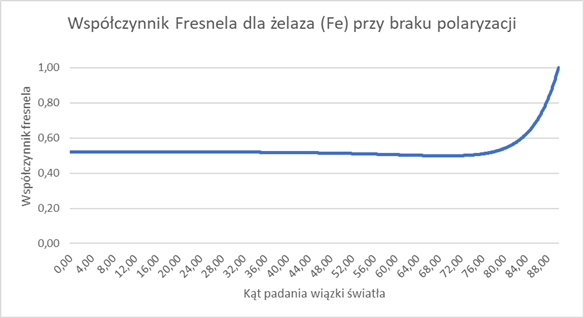
\includegraphics{pbr/fe_fresnel}
    \caption{Współczynnik Fresnela dla żelaza dla niespolaryzowanego światła. Dane pochodzą ze strony \url{https://refractiveindex.info/}}
    \label{fig:fe_fresnel}
\end{figure}

\begin{figure}[h]
    \centering
    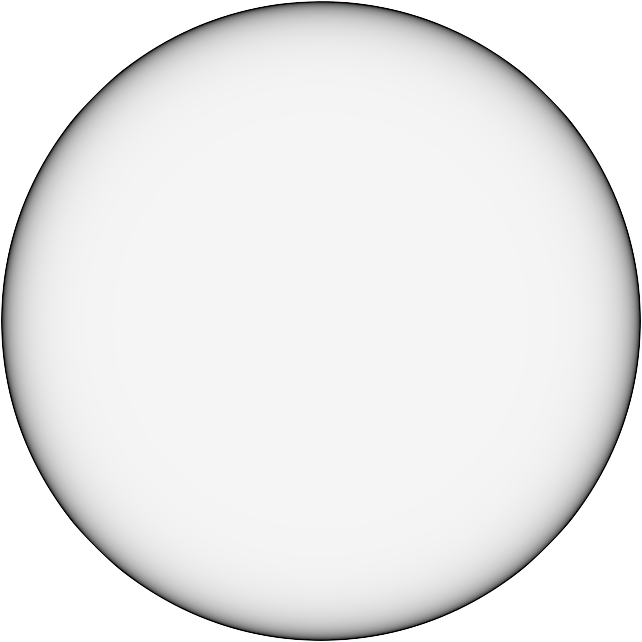
\includegraphics[width=6cm]{pbr/fresnel}
    \caption{Odwrócony współczynnik Fresnela, aproksymacja Schlicka dla $F_0 = 0.04$. Źródło światła znajduje się w tym samym miejscu co obserwator. Opracowanie własne.}
    \label{fig:schlick_fresnel}
\end{figure}

Napopularniejszą metodą wyznaczania przybliżonej wartości współczynnika Fresnela jest aproksymacja Schlicka:
\[
    F_{\text{Schlick}} = F_0 + (1-F_0)(1-\cos\theta)^5
\]
\noindent gdzie $F_0$ jest reflektancją powierzchniową danego materiału zmierzoną pod kątem $\ang{0}$ oraz $\theta = (n \cdot \omega_i)$. Warto zauważyć, że dla przypadku, w którym rozpatrujemy model bazujący na mikropowierzchniach, musimy zastosować wektor połówkowy $m$ zamiast normalnej:
\[
    F_{\text{Schlick}} = F_0 + (1-F_0)\left(
        1 - \left(
            m \cdot \omega_i
        \right)
    \right)^5
\]
\noindent Z definicji wektora połówkowego wynika, że $m \cdot \omega_o = m \cdot \omega_i$ stąd również:
\[
F_{\text{Schlick}} = F_0 + (1-F_0)(1 - (m \cdot \omega_o))^5
\]

Alternatywną metodą aproksymacji jest przybliżenie wykorzystujące sferyczne gaussowskie (ang. \textit{Spherical Gaussian}) \cite{pbr_ue4,SphericalGaussianLegarde}:
\[
    F_{\text{Gauss}} = F_0 +(1−F_0) 2^{\left[
        \left(
            −5.55473\left(\omega_o \cdot m\right)−6.98316
        \right) 
        (\omega_o \cdot m)
  \right]}
\]

\subsection{Funkcja geometryczna}

Funkcja geometryczna (lub zaciemnianie geometryczne, ang. \textit{Geometric
Shadowing}) odpowiada za wspomniane wcześniej zjawiska rzucania cieni w obrębie
mikropowierzchni, w związku z czym światło, które pada pod pewnym kątem nie
odbija się od całości powierzchni (ang. \textit{shadowing}, rys.
\ref{fig:GeometricShadowing}) oraz zasłaniania promieni odbitych od powierzchni
zmierzających do obserwatora przez inne elementy tej powierzchni, w związku z
czym światło odbite nie dociera w całości do obserwatora (ang.
\textit{masking}). W realnym świecie promień po takim zderzeniu nie znika, ale
uproszczone modele traktują takie zachowanie jako absorpcję światła przez
powierzchnię.

Współczynnik związany z zaciemnianiem geometrycznym oznaczymy przez $G(\omega_i,\omega_o,m)$.
Wartość funkcji $G$ określa procent powierzchni skierowanych w kierunku
$m$, które nie są zaciemnione lub zasłonięte.

\begin{figure}[h]
  \centering
  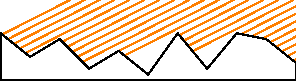
\includegraphics{illustrations/pbr/geometry_shadowing.pdf}
  \vspace{0.25cm}
  \caption{Samozacienianie wewnątrz mikropowierzchni. Opracowanie własne.}
  \label{fig:GeometricShadowing}
\end{figure}

Funkcja geometryczna nazywaną funkcją implicit, która eliminuje czynnik geometryczny zdefiniowana jest poprzez:
\[
  G_{\text{implicit}}(\omega_i, \omega_o, m) =
    (n \cdot \omega_i) (n \cdot \omega_o)
\]

Kolejną możliwą funkcją geometryczną jest funkcja zaproponowana przez Cooka i Torrance'a \cite{CookTorrance}:
\[
  G_{\text{Cook-Torrance}}(\omega_i,\omega_o,m) =
    \min \left(
      1,
      \frac{2(n \cdot m)(n \cdot \omega_o)}{
        \omega_o \cdot m
      },
      \frac{2(n \cdot m)(n \cdot \omega_i)}{
        \omega_o \cdot m
      }
    \right)
\]

Funkcje geometryczne korzystające z metody Smitha polegającej na rozbiciu
funkcji $G$ na dwa niezależne czynniki korzystające z tej samej funkcji $G_1$
z parametrem kolejno $\omega_i$ oraz $\omega_o$, tzn:
\[
  G(\omega_i, \omega_o, m) = G_1(\omega_i) G_1(\omega_o)
\]

Tak jak w poprzednim przypadku istnieje kilka modeli funkcji $G_1$.
Najpopularniejszymi wyborami są: GGX \cite{WalterMicrofacetModels} oraz aproksymacja Schlick-GGX:
\[
  G_{1}^{\text{GGX}}(\omega) =
    \chi^{+}\left(\frac{\omega \cdot m}{\omega \cdot n}\right)
    \frac{2}{
      1 + \sqrt{
        1 + \alpha^2 \tan^{2}\left(\theta_v\right)
      }
    }
\]
\[
  G_{1}^{\text{Schlick-GGX}}(\omega) =
    \frac{n \cdot \omega}{
      (n \cdot \omega)(1 - k) + k
    }
\]
\noindent gdzie $k = \frac{\alpha}{2}$.

\subsection{Podsumowanie}

Powyższe definicje umożliwają nam zbudowanie ogólnego modelu fizycznego
biorącego pod uwagę podstawowe zjawiska zachodzące w mikropowierzchniach,
będących powierzchniami idealnie płaskimi.

W tej pracy będziemy korzystać głównie z funkcji rozkładu normalnych GGX,
aproksymacji Schlicka oraz funkcji geometrycznej GGX.

\todo[inline]{Dodać część diffuse Cook-Torrance}

\section{Swiatła punktowe}

Powszechną optymalizacją w grach komputerowych jest zastępowanie naturalnie występujących świateł powierzchniowych światłami punktowymi \cite{pbr_background}. Swiatła takie nie są fizycznie możliwe, lecz bardzo upraszczają obliczenia i w odpowiedniej skali potrafią bardzo dobrze aproksymować efekty świetlne mimo tego, że są nieskończenie małe.

Podczas lokalnych obliczeń wpływu takiego światła, parametrami jest wektor łączący obecnie badany punkt na powierzchni $p$ oraz centrum źródła $p_l$, którego znormalizowaną postać oznaczamy poprzez $l$ oraz kolor światła $\clightcolor$. Kolor światła $\clightcolor$ zdefiniujemy jako całkowitą odbitą radiancję dla 100\% białego materiału Lambertowskiego z normalną w kierunku zgodnym z kierunkiem wyznaczonym przez $l$, tzn:
\[
	\clightcolor = \frac{1}{\pi} \int_{\Omega} { L_i(\omega_l) (l \cdot \omega_i) \dd\omega_i }
\]

Załóżmy teraz, że w scenie występuje dokładnie jedno światło powierzchniowe o bardzo małej powierzchni. Całe światło jest zawarte w stożku o osi obrotowej leżącej na $l$ oraz o środku w punkcie $p$ o rozmiarze kątowym $\epsilon$. Dla pozostałych kierunków niezawartych w tym stożku radiancja jest zerowa. Przy założeniu, że $\clightcolor$ się nie zmienia oraz $\epsilon$ może być dowolnie mały otrzymujemy:
\[
	\clightcolor = \frac{1}{\pi} \lim_{\epsilon \rightarrow 0} \left(
		\int_{\Omega} { L_i(\omega_l) } \dd\omega_i
	\right)
	\Rightarrow
	\lim_{\epsilon \rightarrow 0} \left(\int_{\Omega} { L_i(\omega_l) } \dd\omega_i \right) = \pi\clightcolor
\]

Postępując analogicznie z równaniem renderingu otrzymujemy:
\[
	L_o(\omega_o) = \lim_{\epsilon \rightarrow 0} \left(
		\int_{\Omega}{ f(\omega_i, \omega_o) L_i(\omega_i) (n \cdot \omega_i) } \dd\omega_i
	\right) =
	 f(l, \omega_o) \lim_{\epsilon \rightarrow 0} \left(
	 	\int_{\Omega} { L_i(\omega_l) } \dd\omega_i
	 \right)
	 (n \cdot l)
\]

Podstawiając za całkę stałą $\clightcolor$ otrzymujemy:
\[
	L_o(\omega_o) = \pi f(l, \omega_o) \clightcolor (n \cdot l)
\]

Jak widać, powyższe równanie aproksymuje obliczenie skomplikowanego wyrażenia całkowego jednokrotnym obliczeniem funkcji BRDF oraz kilkoma prostymi operacjami arytmetycznymi. Pozostaje pytanie, kiedy warto zastosować tego typu technikę. Aproksymacja ta, ma sens dla dynamicznych scen w których precyzja nie jest kluczowa oraz odległość od źródła światła jest co najmniej pięć razy większa od jego szerokości \cite{RealTimeRendering2008,lambert_photometria} - w takim przypadku konwersja na światło punktowe wraz z kwadratowym spadkiem intensywności powinna być wystarczająca w grach.


\section{Przybliżenie światła powierzchniowego klastrem świateł punktowych}

Pierwszą metodą, która nasuwa się po poznaniu podstaw, jest podejście uproszczone polegające na przybliżeniu klasycznego światła powierzchniowego zbiorem świateł punktowych.

Będziemy badać światła powierzchniowe tego typu w formie prostokątnej ze względu na łatwość generowania jednorodnej siatki punktów wewnątrz takiego obszaru, kształt ten również posiada ostre krawędzie i rogi przez co minusy tej metody będą bardzo widoczne. Uogólnienie do dowolnego kształtu nie będzie wpływać na rezultaty jakościowo.

Załóżmy, że mamy prostokątne światło powierzchniowe o stałej irradiancji $E$ niezależnej od wybranego punktu. Wygenerujemy na nim siatkę jednakowych świateł punktowych z zastrzeżeniem, że działają one tylko gdy zachodzi warunek $n \cdot \omega_i > 0 $. To znaczy zakładamy, że światło powierzchniowe jest jednostronne.

Siatka punktowa będzie wygenerowana w taki sposób, aby każdy punkt przybliżał jednakowy fragment powierzchni światła (rys. \ref{fig:PointLightCluster}).

\begin{figure}[ht]
  \centering
  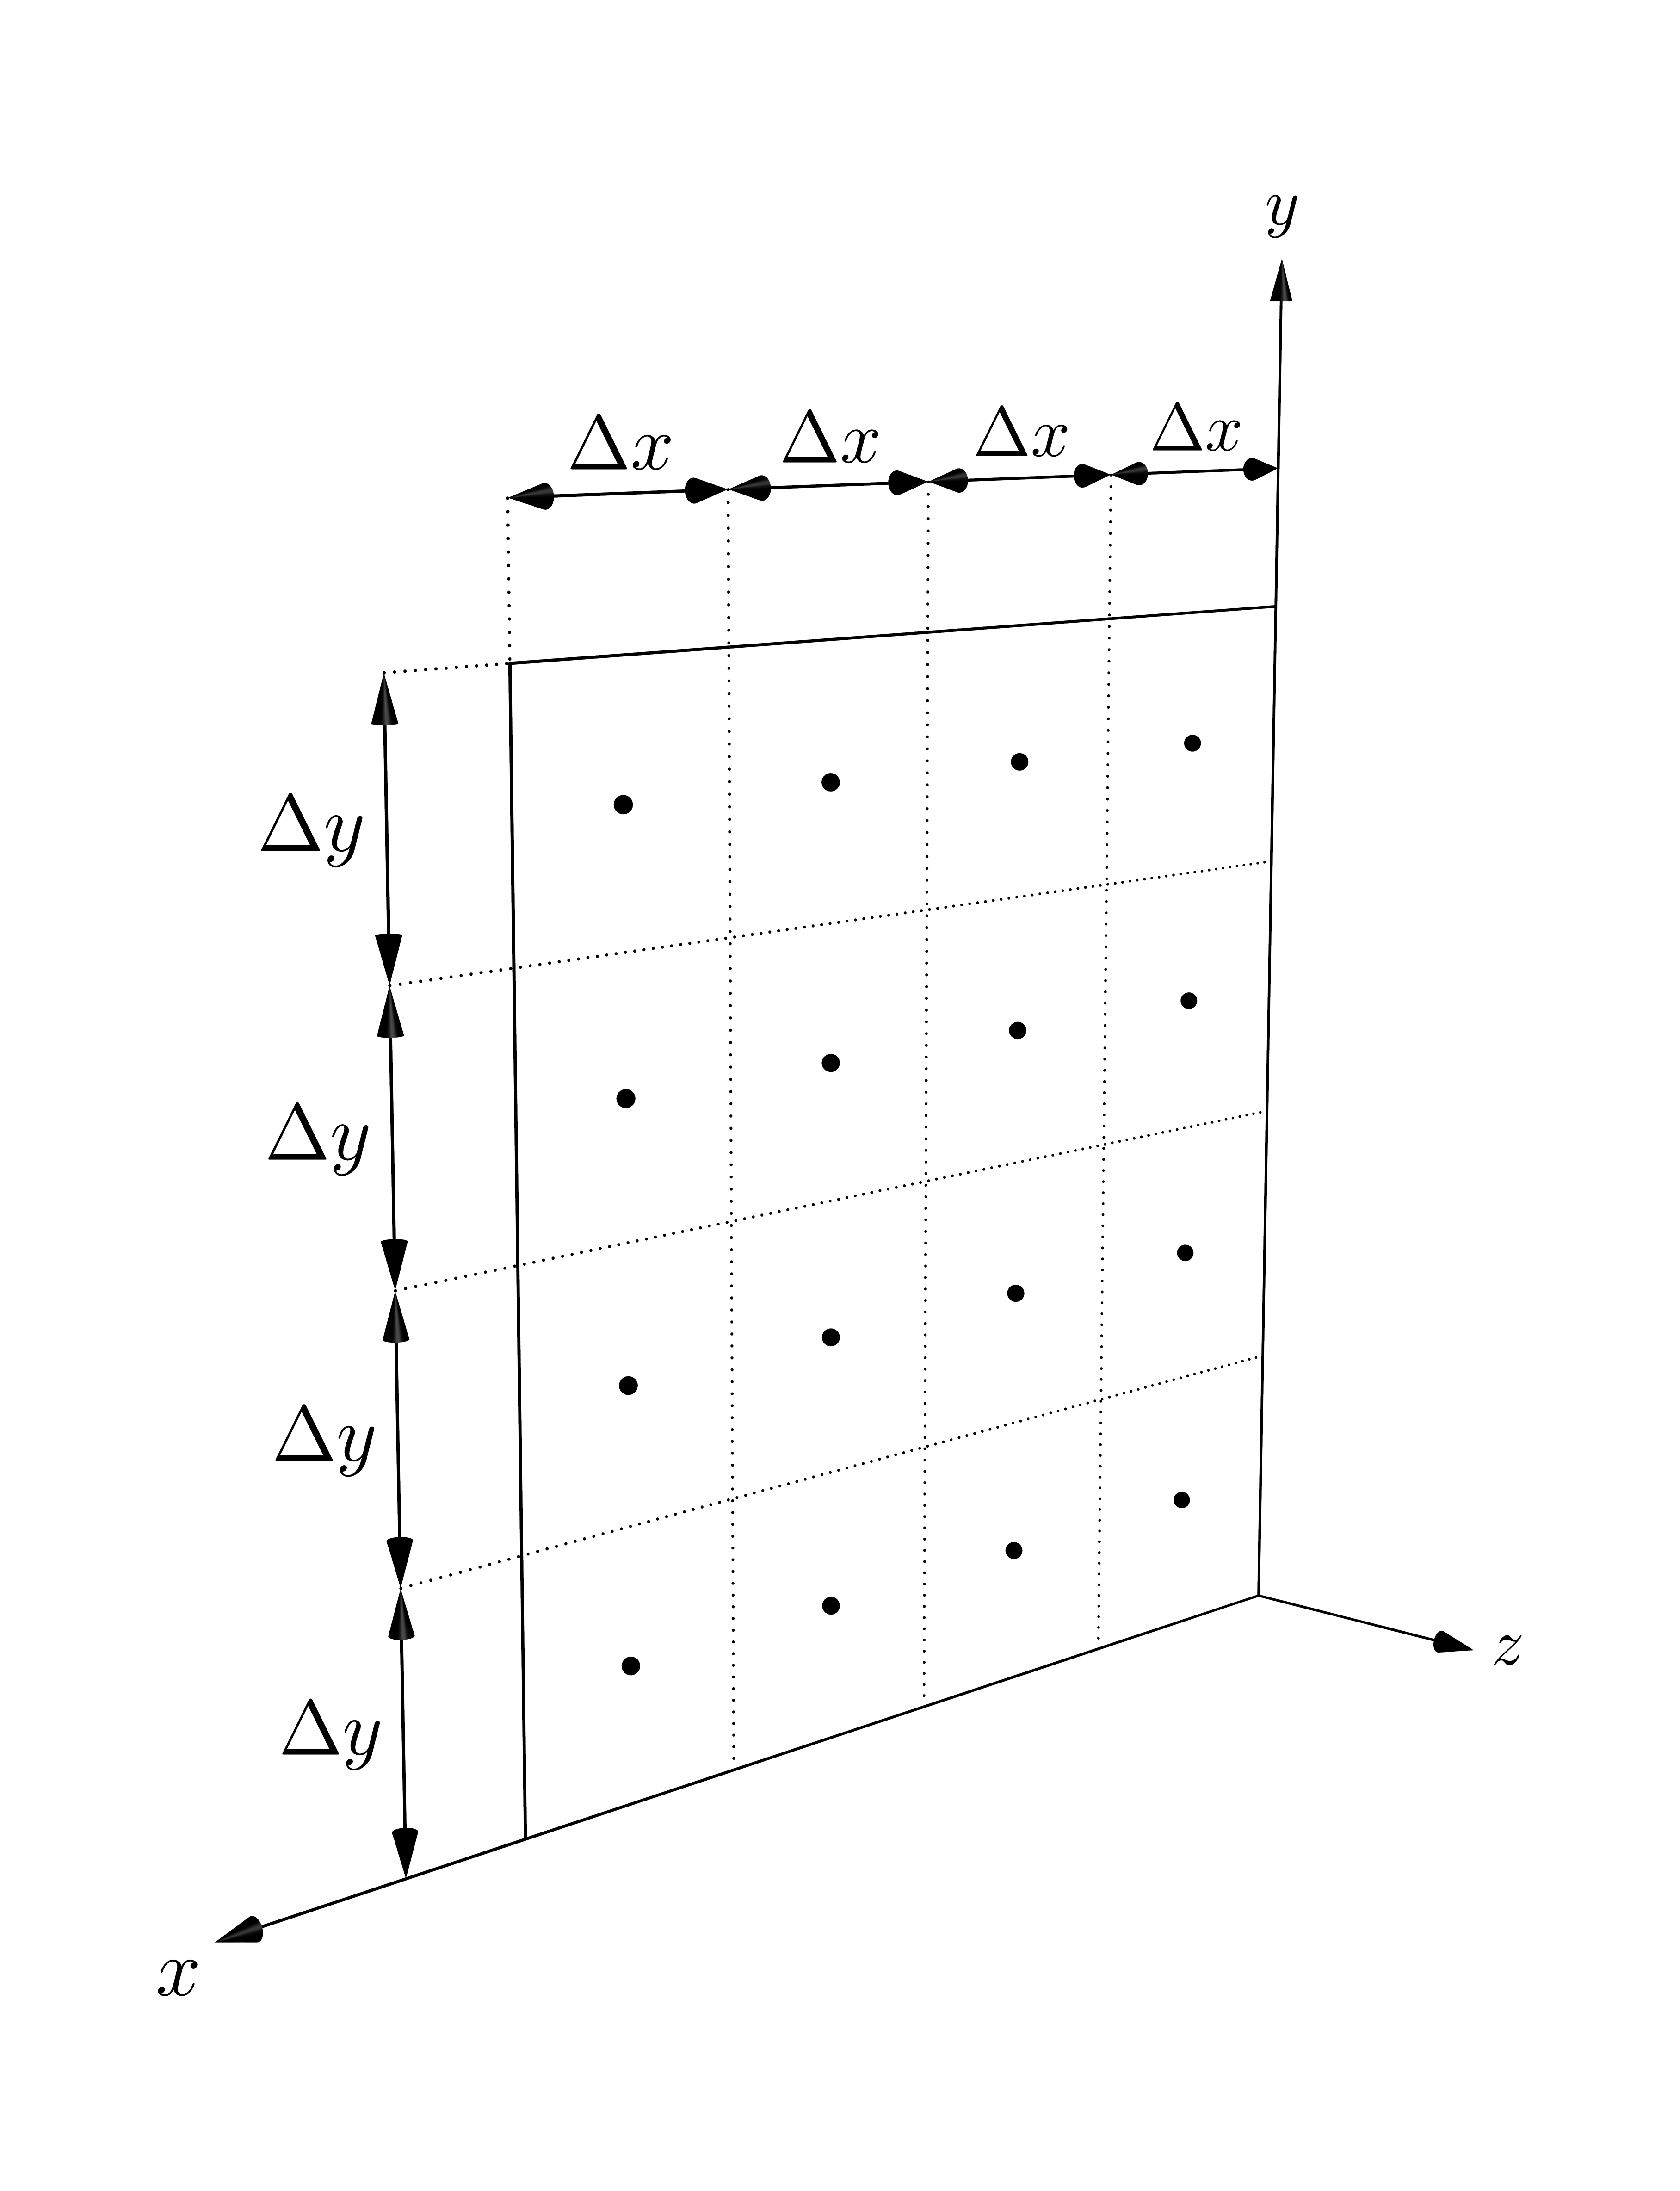
\includegraphics[height=10cm]{pbr/light_cluster.png}
  \caption{Klaster świateł punktowych na świetle powierzchniowym. Opracowanie własne.}
  \label{fig:PointLightCluster}
\end{figure}

Energię promieniowania dla tak zdefiniowanego przypadku możemy obliczyć korzystając z definicji irradiancji:
\[
	\Phi = E \Delta{x} \Delta{y}
\]

Intensywność takiego źródła jest stała (dla danej długości fali $\lambda$) i równa: 

\[
  I 
	= \lim_{\Delta\omega \rightarrow 0} {
		\frac{\Delta\Phi}{\Delta\omega}
	} 
	= \frac{\Phi}{2\pi}
	= \frac{E\Delta{x}\Delta{y}}{2\pi}
\]

Korzystając z wcześniejszych definicji dla punktu $p$ na powierzchni i światła punktowego o środku w $l_c$ otrzymujemy \cite{pbr_frostbite}:
\[
	L_o(\omega_o) = \pi f(l, \omega_o) \frac{I}{r^2} (n \cdot l)
\]

\noindent gdzie $r$ jest równe $\norm{p-l_c}$.

Zatem dla całego klastra, wystarczy zsumować wpływ każdego ze świateł punktowych opisujących podobszary:
\[
	L_o(\omega_o) = \pi \sum_{i}^{n} \sum_{j}^{m} {
		f(l_{i,j}, \omega_o) \frac{I}{(r_{i,j})^2} (n \cdot l_{i,j})
	}
\]

\end{document}
